\section{Durchführung}
\label{sec:Durchführung}

Für die Messung wurde eine Grundplatte wie in \autoref{fig:Abb1} dargestellt benutzt. Genauere Daten der Probestäbe wurden in der \autoref{tab:werte2} angegeben.

\begin{figure}
    \centering
    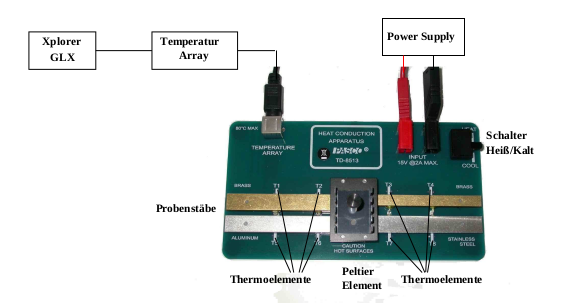
\includegraphics[scale=0.7]{content/Bilder/Aufbau.png}
    \caption{Hier zu sehen ist die für das Experiment verwendete Grundplatte, dessen Probestäbe im Verlauf des Versuchs aufgeheizt und abgekühlt wurden. Die einzelnen Bauteile sind hier beschrieben.}
    \label{fig:Abb1}
\end{figure}

\begin{figure}
    \centering
    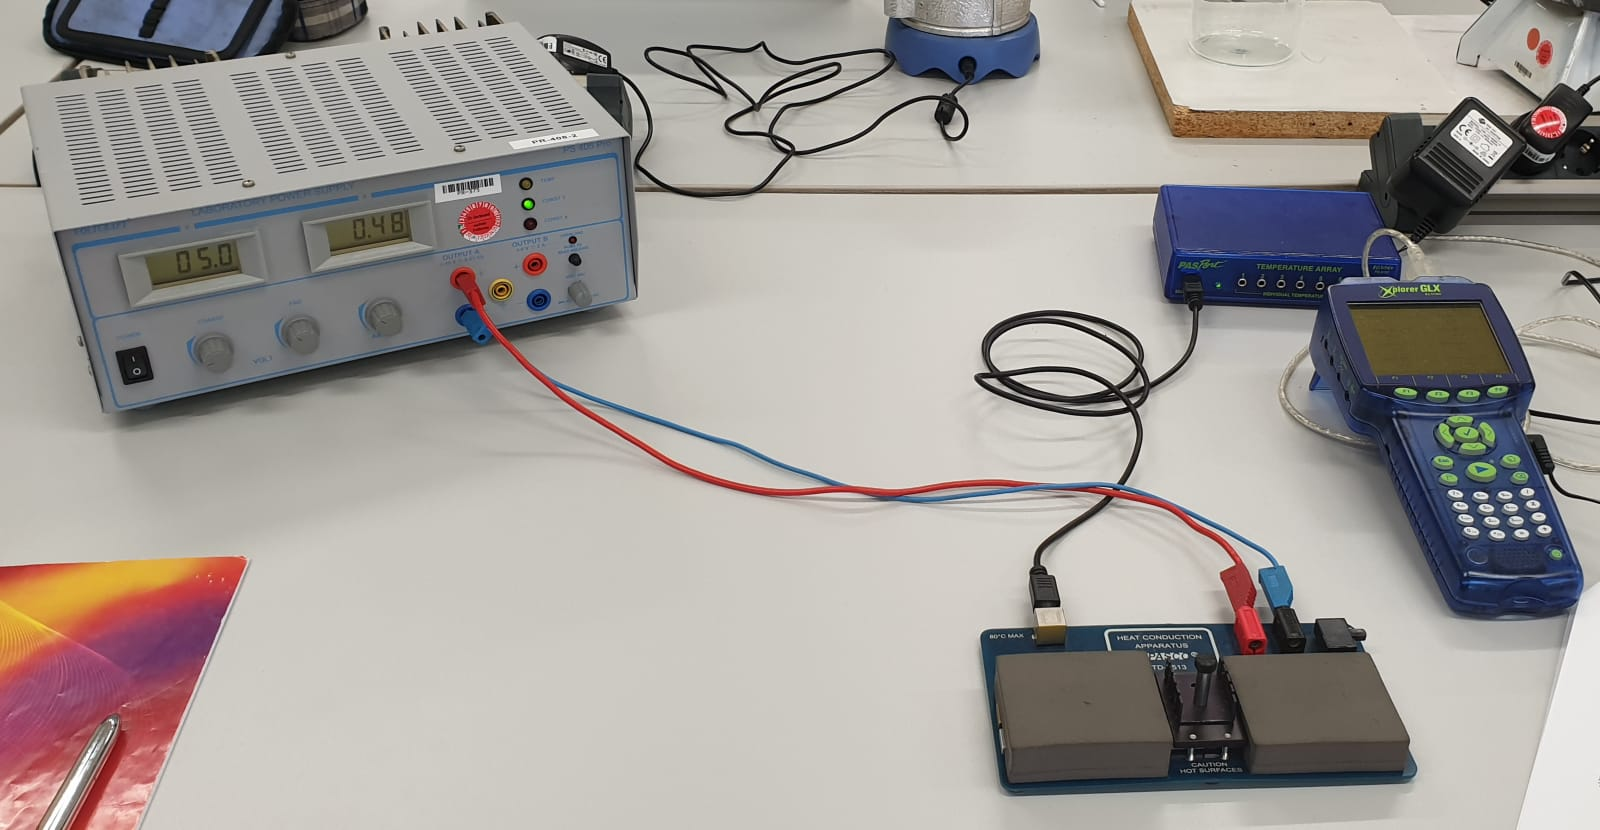
\includegraphics[scale=0.2]{content/Bilder/Aufbau2.png}
    \caption{Diese Abbildung visualisiert, wie das Experiment aufgebaut wurde. Links oben ist die Spannungsquelle, der Power Supply, zu sehen. Im Vordergrund die Grundplatte, rechts im Vordergrund das für die Messung verwendete GLX und dahinter das Temperatur Array.}
    \label{fig:Abb2}
\end{figure}

\begin{table}
    \centering
    \caption{Hier ist eine Auflistung für die gegebenen Werte der Bauteile des Schwingkreises.}
    \label{tab:werte2}
    \begin{tabular}{c|c|c|c}
        Material & Abmessungen [cm] & $\rho$ [$\frac{kg}{m^3}$] & $c$ [$\frac{J}{kg\cdot K}$]\\
        \midrule
        Messing (breit) & 9 x 1.2 x 0.4 & 8520 & 385\\
        Messing (schmal) & 9 x 0.7 x 0.4 & 8520 & 385\\
        Aluminium & 9 x 1.2 x 0.4 & 2800 & 830\\
        Edelstahl & 9 x 1.2 x 0.4 & 8000 & 400\\
    \end{tabular}
  \end{table}

Weiterhin wird für Messzwecke ein Temperatur-Array ein GLX und eine Spannungsquelle. Der Versuch wird wie in \autoref{fig:Abb2} aufgebaut und nun auf zwei verschiedenen Weisen durchgeführt.

\subsection{Statische Methode}
  Die statistische Methode gibt vor, an zwei verschiedenen auf der Grundplatte markierten Stellen die Temperatur als Funktion der Zeit zu messen.\\
  Dazu wird zunächst die Spannungsquelle auf 5V und der Strom auf maximaler Amplitude eingestellt. Auf dem GLX wird die Abtastrate auf 5 Sekunden gesetzt und abgewartet, bis die Temperatur des Thermoelements \(T_7\) 45°C erreicht. Danach wird der Schalter auf der Grundplatte von "HEAT" auf "COOL" geschaltet und die Stäbe abgekühlt.\\
  Die Temperaturen an den Thermoelementen \(T_1\), \(T_4\), \(T_5\) und \(T_8\) werden aufgezeichnet. Das Abkühlen geht weiter, bis die Thermoelemente in etwa 30°C erreichen.\\
  Zum Schluss werden Grafiken für |\(T_7\)-\(T_8\)| und |\(T_2\)-\(T_1\)| als Funktion der Messzeit \(t\) erstellt und der Wärmestrom nach \autoref{eq:warmcurrent} berechnet.
  
\subsection{Dynamische Methode}
  Nun wird die Spannung bis auf 8 Volt erhöht. Im Gegensatz dazu bleiben alle anderen Einstellungen unverändert.\\
  Im nächsten Experiment werden die Probenstäbe T-Periodisch aufgeheizt und abgekühlt.\\
  Zuerst wird alle 40 Sekunden erwärmt und gekühlt. Dies mindestens 10 Mal. Daraufhin folgt eine Abkühlung, sodass die Temperaturen der Stäbe ca. 30°C betragen. Zum Schluss des Experiments werden die Stäbe alle 200 Sekunden erhitzt und gekühlt, bis der heißeste Stab eine Temperatur von 80°C erreicht. Auch dies wird graphisch ausgegeben. Die Absicht hierbei ist es die Wärmeleitfähigkeit \(\kappa\) mithilfe von \autoref{eq:warleit} zu ermitteln.